\documentclass[a4paper]{article}
\usepackage[utf8]{inputenc}
\usepackage[russian,english]{babel}
\usepackage[T2A]{fontenc}
\usepackage[left=10mm, top=20mm, right=18mm, bottom=15mm, footskip=10mm]{geometry}
\usepackage{indentfirst}
\usepackage{amsmath,amssymb}
\usepackage[italicdiff]{physics}
\usepackage{graphicx}
\usepackage{siunitx}
\graphicspath{{images/}}
\DeclareGraphicsExtensions{.pdf,.png,.jpg,.jpeg}
\usepackage{wrapfig}

\usepackage{caption}
\captionsetup[figure]{name=Рисунок}
\captionsetup[table]{name=Таблица}

\title{\underline{Вопрос по выбору (Электричество и магнетизм)}}
\author{Воронин Денис, Б04-407}
\date{}
\begin{document}

\maketitle
\begin{center}
\textbf{\Large Принципы радиосвязи}
\end{center}

\section{Начальные сведения}

Каждый провод, по которому течет переменный ток, излучает  э-м волны. Но если ток замкнут и выполнено условие квазистационарности,
то издучения практически не будет. \par
Разобъем провод на элементы тока $\mathcal{J} dl$. Каждый такой элемент излучает как точечныый диполь, производная дипольного момента которого:
\[\overrightarrow{p'}=\oint d \overrightarrow{p'} =\oint \mathcal{J}d\overrightarrow{l} \stackrel{\text{квазистац.}}{=}\mathcal{J}\oint d\overrightarrow{l} = 0\] 

При более точном рассмотрении замкнутый виток с током можно разбить на две половины и каждую из них заменить точечным диполем.\par
Для получения интенсивного излучения надо перейти к открытым системам, в которых токи не замкнуты. Такой системой является прямолинейный провод, в котором возбуждаются незамкнутые переменные токи.\par
В радиотехнике издучающей системой служит антенна - незамкнутый провод или система проводов, подвешенных высоко над землей, по которым текут переменные токи.\par
Низкочастотные токи не годятся, т.к. они излучают очень слабо и для возбуждения сильных колебаний нужны большие размеры антенны.\par
\textbf{Принцип радиосвязи}: 


\begin{wrapfigure}{l}{0.4\textwidth}
    \centering
    
\includegraphics[width=0.38\textwidth]{pick1.png}
    \caption{Принцип радио связи}
    \label{fig:example}
\end{wrapfigure}
В антенне передающей радиостанции возбуждаются сильные высокочастотные токи. Э-м волны из передающей антенны, достигая приемной антенны, возбуждают в ней токи той же частоты, которые могут быть усилены и использованы. Для настройки антенн конденсатор можно включать последовательно к катушке индуктивности(при параллельном соед. увелич общая емкость системы, значит ее собственная частоты уменьшается, а при последовательном 
соединении наоборот)

\section{Решение проблем с помощью модуляции}

Волны высокой частоты не воспринимаются ухом человека, а также не несут никакой информации. Для передачи информации требуются низкочастотные сигналы, но их передача невозможна. Эта решается с помощью передачи синусоидальными волнами высокой частоты, измененными низкочастотными сигналами. Это называется \textbf{модуляцией}, а сами волны \textbf{модулированными}. 
Далее будем рассматривать амплитудную модуляцию.\par

Если нет передачи сигнала:
\[\mathcal{J} = \mathcal{J}_{0}sin(\omega t)\]

Если есть передача:
\[\mathcal{J} = \mathcal{J}_{0}[1+f(t)]sin(\omega t)\]

Функция f(t) - модулирующая функция, зависит от формы передаваемого (модулирующего сигнала) $\left\lvert f(t)\right\rvert <1$.\par

Простая модулирующая функция соответсвует передаче только музыкального тона (камертон). Тогда 
\[f(t) = msin(\Omega t)\]

где $\Omega$ - частота, а m - глубина модуляции.\par

Подставляя f(t) в формулу получим:

\[\mathcal{J} = \mathcal{J}_{0}[1+msin(\Omega t)]sin(\omega t) \stackrel{\text{sin*sin}}{=} \mathcal{J}_{0}sin(\omega t) + \frac{m\mathcal{J}_{0}}{2}cos(\omega - \Omega)t - \frac{m\mathcal{J}_{0}}{2}cos(\omega + \Omega)t\]

Если f(t) не синусоидальна, но периодична, то ее можно разложить в ряд Фурье и к каждому члену этого разложения применить рассуждение выше. Тогда вместо 2-х частот $\omega - \Omega$ и $\omega + \Omega$ слева и справа от $\omega$ появится еще несколько боковых частот.
Они образуют боковые полосы, состоящие из дискр набора частот. Если f(t) не периодична то она раскладывается в интеграл Фурье. 

\begin{figure}[h]
    \centering
    
\includegraphics[width=0.4\textwidth]{pick2.png}
    \caption{Модуляция}
    \label{fig:example}
\end{figure}

\section{Прием модулированных колебаний}
\begin{wrapfigure}{l}{0.4\textwidth}
    \centering
    
\includegraphics[width=0.38\textwidth]{pick3.png}
    \caption{Возможная схема детектирования}
    \label{fig:example}
\end{wrapfigure}
Модулированная волна передающей антенны возбуждает в приемной антенне такие же модулированные, но более слабые колебания.
Даже после предварительного усиления они ще не годятся для воспроизведения. Причиной этому служит то, что модулированные колебания, если их разложить на синусоидальные составляющие будут содержать только высокие частоты.
\par
Поэтому принятый сигнал нужно демодулировать или детектировать.
\textbf{Демодуляция} - это выпрямление с дальнейшим сглаживанием высокочастотных колебаний.

Выпрямление происходит с помощью кристалического детектора D, сгалживание с помощью RC-цепи.  
Пример раюоты детектирующей схемы представлен на рисунке ниже 

		\begin{figure}[h]
			\begin{minipage}[h]{0.5\linewidth}
				\center{
\includegraphics[width=0.9\linewidth]{pick4.png}}
				\caption{Прямоугольные импульсы}
			\end{minipage}
			\begin{minipage}[h]{0.5\linewidth}
				\center{
\includegraphics[width=0.9\linewidth]{pick5.png}}
				\caption{Прямоугольные импульсы}
			\end{minipage}
		\end{figure}
	
\newpage

\textbf{Итогвую схему} работы приемника можно представить в виде следующей блоксхемы:

\begin{figure}[h]
    \centering
    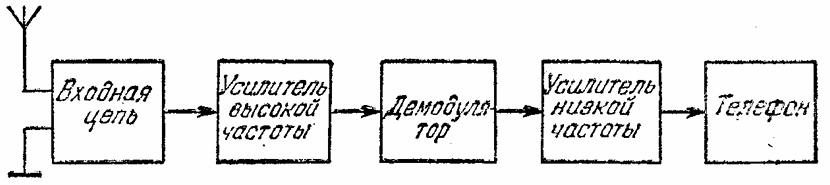
\includegraphics[width=0.6\textwidth]{pick6.png}
    \caption{Схема работы}
    \label{fig:example}
\end{figure}

\section{Простейший вариант радиоприемника}

Для приема сигналов порядка нескольких метров достаточно реализовать следующую схему устройства:

\begin{figure}[h]
    \centering
    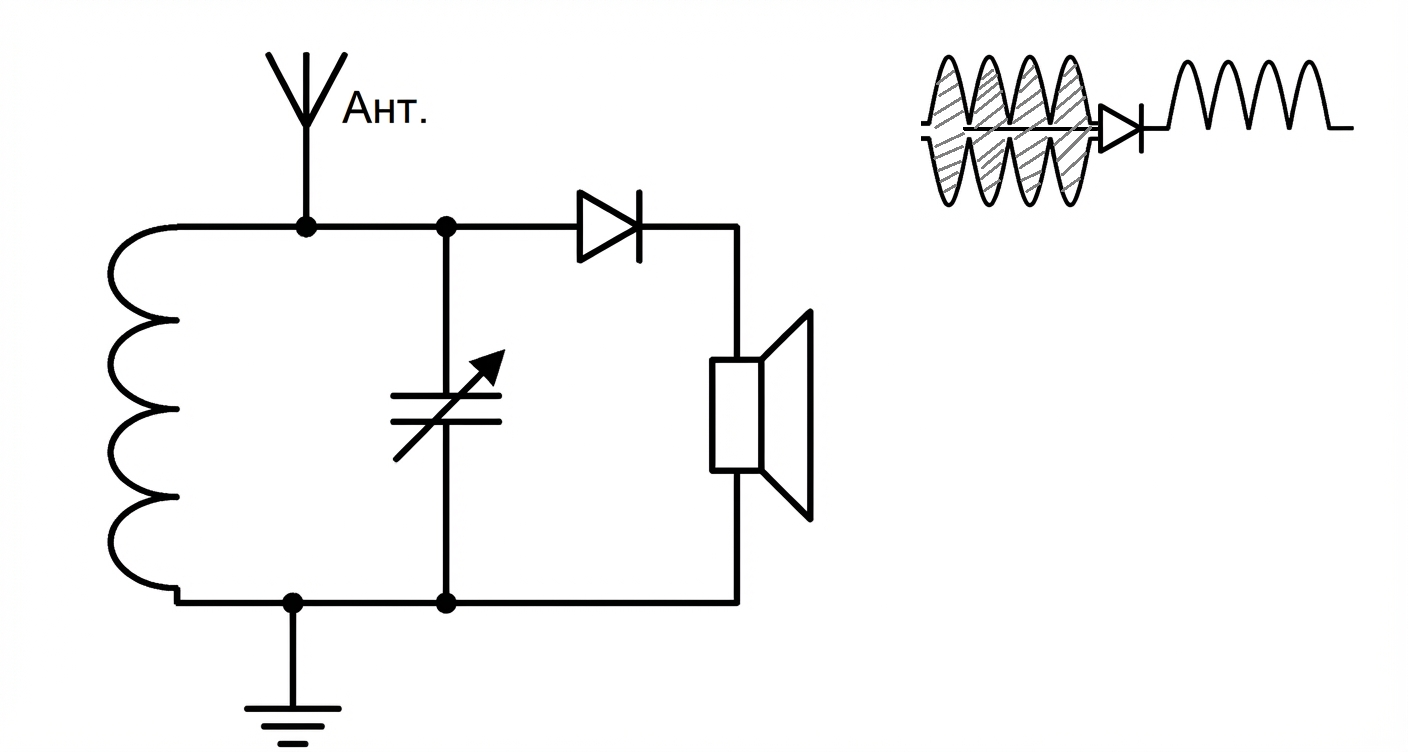
\includegraphics[width=0.6\textwidth]{Radio_sketch.png}
    \caption{Схема работы}
    \label{fig:example}
\end{figure}

Практическая реализация приемника: 

\begin{figure}[h]
    \centering
    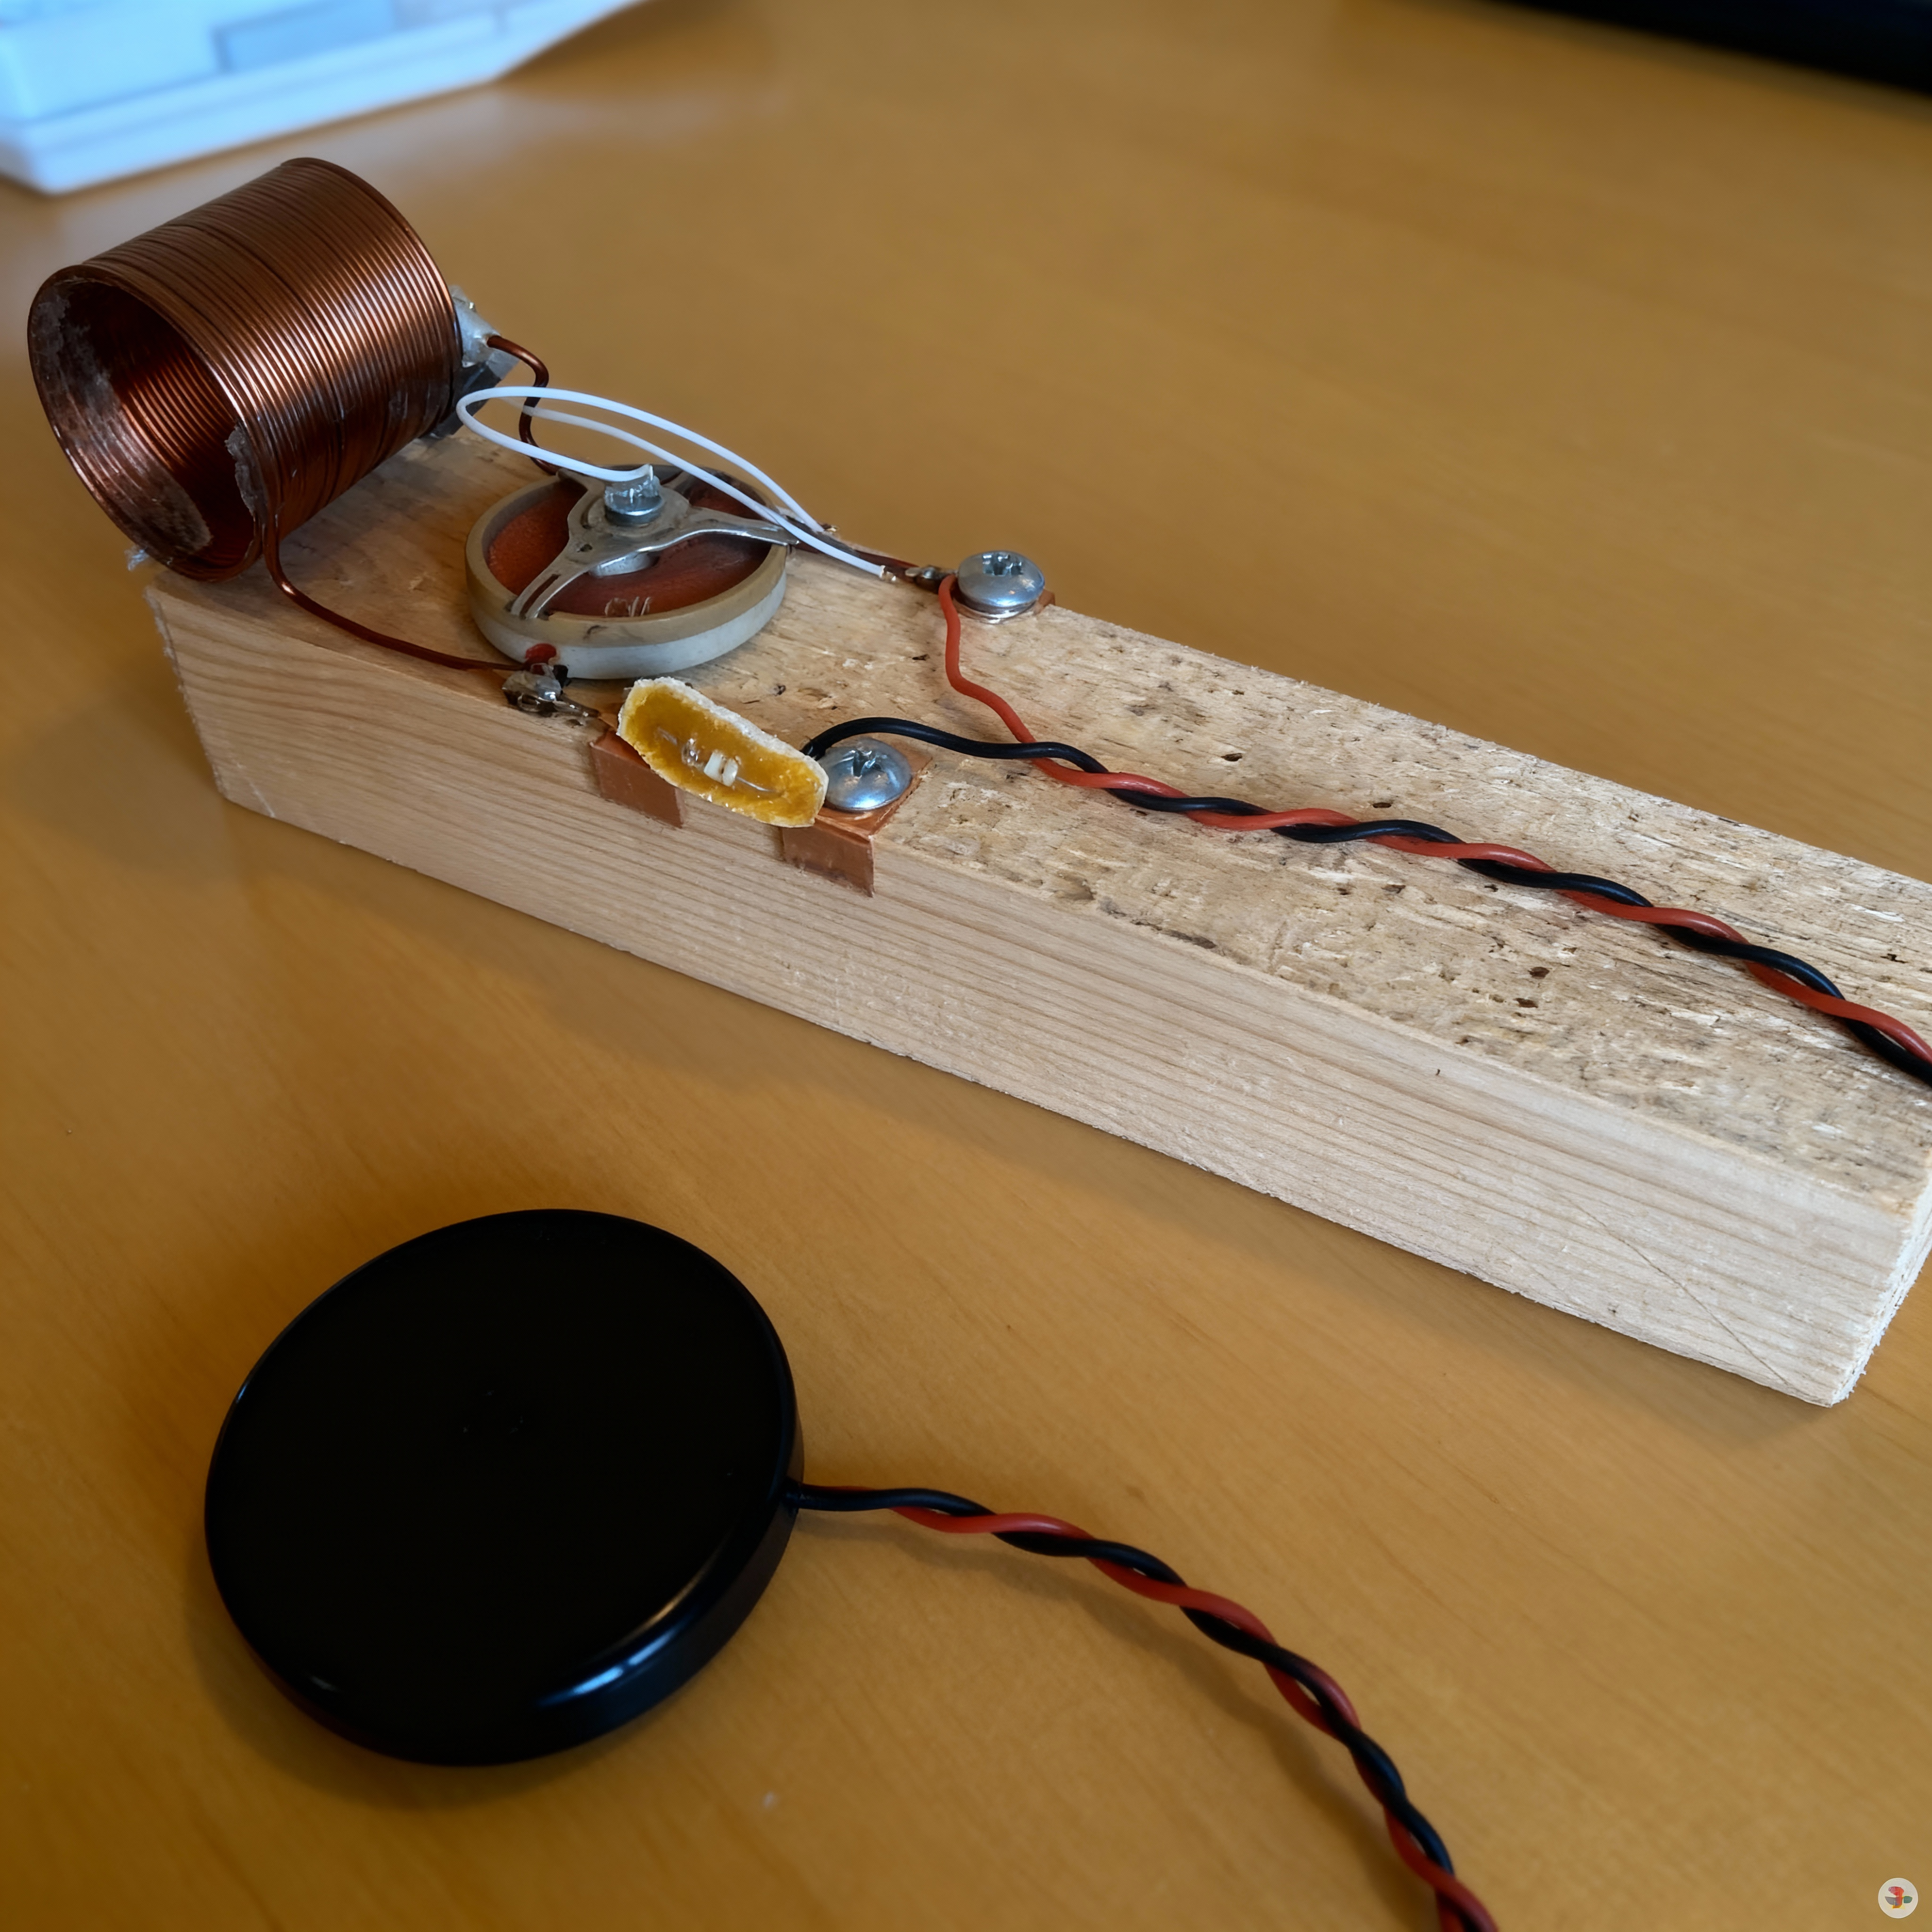
\includegraphics[width=0.45\textwidth]{Radio.jpeg}
    \caption{Практическая реализация}
    \label{fig:example}
\end{figure}

\newpage

\section{Рассчет длины антенны для детекторного радиоприемника}

\subsection{Рассчитаем индуктивность катушки}

\textbf{Катушка:}
\begin{itemize}
    \item Число витков: $N = 20$
    \item Радиус витка: $r = 2~\text{см} = 0.02~\text{м}$
    \item Диаметр проволоки: $d = 1~\text{мм} = 0.001~\text{м}$
\end{itemize}

\textbf{Длина намотки катушки:}
\[
l_{\text{катушки}} = N \cdot d = 20 \cdot 0.001 = 0.02~\text{м}
\]

\textbf{Площадь витка:}
\[
S = \pi r^2 = \pi \cdot (0.02)^2 \approx 1.2566 \cdot 10^{-3}~\text{м}^2
\]

\textbf{Индуктивность однослойной катушки (приближенно):}
\[
L = \frac{\mu_0 N^2 S}{l_{\text{катушки}}}
\]
где $\mu_0 = 4\pi \cdot 10^{-7}~\text{Гн/м}$ — магнитная постоянная.

\[
L = \frac{4\pi \cdot 10^{-7} \cdot 20^2 \cdot 1.2566 \cdot 10^{-3}}{0.02}
\]

\[
L \approx \frac{4\pi \cdot 10^{-7} \cdot 400 \cdot 1.2566 \cdot 10^{-3}}{0.02}
\]

\[
L \approx \frac{4\pi \cdot 5.0264 \cdot 10^{-7}}{0.02} \approx \frac{6.317 \cdot 10^{-6}}{0.02} \approx 3.158 \cdot 10^{-4}~\text{Гн}
\]

\[
L \approx 31.58~\text{мкГн}
\]

\subsection{Резонансная частота контура}

\textbf{Резонансная частота:}
\[
f_0 = \frac{1}{2\pi \sqrt{LC}}
\]

\textbf{Конденсатор переменной емкости:} $C_{\min} = 5~\text{пФ},\quad C_{\max} = 20~\text{пФ}$

\textbf{Для $C_{\min} = 5~\text{пФ}$:}
\[
f_{\max} = \frac{1}{2\pi \sqrt{31.58 \cdot 10^{-6} \cdot 5 \cdot 10^{-12}}}
\]

\[
\sqrt{LC} = \sqrt{31.58 \cdot 10^{-6} \cdot 5 \cdot 10^{-12}} = \sqrt{1.579 \cdot 10^{-16}} \approx 1.257 \cdot 10^{-8}
\]

\[
f_{\max} \approx \frac{1}{2\pi \cdot 1.257 \cdot 10^{-8}} \approx \frac{1}{7.896 \cdot 10^{-8}} \approx 1.266 \cdot 10^{7}~\text{Гц}
\]

\[
f_{\max} \approx 12.66~\text{МГц}
\]

\textbf{Для $C_{\max} = 20~\text{пФ}$:}

\[
f_{\min} = \frac{1}{2\pi \sqrt{31.58 \cdot 10^{-6} \cdot 20 \cdot 10^{-12}}}
\]

\[
\sqrt{LC} = \sqrt{31.58 \cdot 10^{-6} \cdot 20 \cdot 10^{-12}} = \sqrt{6.316 \cdot 10^{-16}} \approx 2.513 \cdot 10^{-8}
\]

\[
f_{\min} \approx \frac{1}{2\pi \cdot 2.513 \cdot 10^{-8}} \approx \frac{1}{1.579 \cdot 10^{-7}} \approx 6.33 \cdot 10^{6}~\text{Гц}
\]

\[
f_{\min} \approx 6.33~\text{МГц}
\]


Значит приемник может работать в диапазоне:
\[
f \approx 6.33~\text{МГц} \quad \text{до} \quad 12.66~\text{МГц}
\]
Это коротковолновый диапазон (КВ).

\newpage

\subsection{Расчет длины антенны для резонанса}

Для эффективного приема антенна должна быть согласована с длиной волны принимаемого сигнала. Оптимальная длина — $\lambda/4$ или $\lambda/2$ (четвертьволновая или полуволновая антенна).

\[
\lambda = \frac{c}{f}, \quad c = 3 \cdot 10^{8}~\text{м/с}
\]

\textbf{Для $f_{\min} = 6.33~\text{МГц}$:}
\[
\lambda_{\max} = \frac{3 \cdot 10^{8}}{6.33 \cdot 10^{6}} \approx 47.4~\text{м}
\]

\textbf{Для $f_{\max} = 12.66~\text{МГц}$:}
\[
\lambda_{\min} = \frac{3 \cdot 10^{8}}{12.66 \cdot 10^{6}} \approx 23.7~\text{м}
\]

Из-за влияния земли и конечной толщины антенны её эффективная длина уменьшается:
\[
l_{\text{эфф}} = k \cdot l_{\text{теор}}
\]
где $k \approx 0.95$ для тонких проводов на высоте.

Для коротковолнового диапазона обычно используют антенну длиной около $10\text{--}15~\text{м}$, что соответствует $\lambda/4$ для средних частот диапазона.

Для данного приемника рекомендована антенна длиной $\approx 10~\text{м}$, что позволит принимать станции в диапазоне $6\text{--}13~\text{МГц}$ с настройкой конденсатором.

\section{Рассчет спектра амплитудно модулированного сигнала}

Рассмотрим амплитудную модуляцию (AM), используемую в детекторном приёмнике. Исходный сигнал описывается выражением:
\[
J(t) = J_0 \left[1 + f(t)\right] \sin(\omega t)
\]
где:
\begin{itemize}
    \item $J_0$ — амплитуда тока несущей,
    \item $\omega = 2\pi f$ — круговая частота несущей ($f$ — несущая частота),
    \item $f(t)$ — модулирующий сигнал (низкочастотный), причём $|f(t)| < 1$.
\end{itemize}

\subsection{Случай тональной модуляции (камертон)}

Пусть модулирующий сигнал — синусоидальный тон:
\[
f(t) = m \sin(\Omega t)
\]
где:
\begin{itemize}
    \item $m$ — глубина модуляции ($0 < m \leq 1$),
    \item $\Omega = 2\pi F$ — круговая частота модулирующего сигнала ($F$ — частота звука, например, $1~\text{кГц}$).
\end{itemize}

Тогда модулированный сигнал:
\[
J(t) = J_0 \left[1 + m \sin(\Omega t)\right] \sin(\omega t)
\]

Раскроем скобки:
\[
J(t) = J_0 \sin(\omega t) + J_0 m \sin(\Omega t) \sin(\omega t)
\]

Используем тригонометрическое тождество:
\[
\sin \alpha \sin \beta = \frac{1}{2} \left[ \cos(\alpha - \beta) - \cos(\alpha + \beta) \right]
\]

Получим:
\[
J(t) = J_0 \sin(\omega t) + \frac{J_0 m}{2} \cos\left[(\omega - \Omega)t\right] - \frac{J_0 m}{2} \cos\left[(\omega + \Omega)t\right]
\]

\subsection{Спектральный состав AM-сигнала}

Сигнал состоит из трёх гармонических компонент:

\begin{enumerate}
    \item \textbf{Несущая:} \\
        Частота: $\omega$, \\
        Амплитуда: $J_0$.
    
    \item \textbf{Нижняя боковая полоса (НБП):} \\
        Частота: $\omega - \Omega$, \\
        Амплитуда: $\dfrac{J_0 m}{2}$.
    
    \item \textbf{Верхняя боковая полоса (ВБП):} \\
        Частота: $\omega + \Omega$, \\
        Амплитуда: $\dfrac{J_0 m}{2}$.
\end{enumerate}

\subsection{Случай периодического модулирующего сигнала}

Если $f(t)$ — периодическая несинусоидальная функция с периодом $T = \dfrac{2\pi}{\Omega_0}$, её можно разложить в ряд Фурье:
\[
f(t) = \sum_{n=1}^{\infty} \left[ a_n \cos(n\Omega_0 t) + b_n \sin(n\Omega_0 t) \right]
\]

Каждая гармоника $n\Omega_0$ создаёт пару боковых частот: $\omega \pm n\Omega_0$.

Тогда спектр AM-сигнала будет состоять из:
\begin{itemize}
    \item Несущей на частоте $\omega$,
    \item Боковых полос на частотах $\omega \pm n\Omega_0$ для $n = 1, 2, 3, \dots$
\end{itemize}

Амплитуды боковых составляющих будут пропорциональны коэффициентам Фурье $a_n$, $b_n$.

\subsection{Численный пример для детекторного приёмника}

Возьмём параметры:
\begin{itemize}
    \item Несущая частота: $f = 10~\text{МГц}$ ($\omega = 2\pi \cdot 10^{7}~\text{рад/с}$),
    \item Частота модуляции: $F = 1~\text{кГц}$ ($\Omega = 2\pi \cdot 10^{3}~\text{рад/с}$),
    \item Глубина модуляции: $m = 0.8$,
    \item Амплитуда тока: $J_0 = 1~\text{мА}$.
\end{itemize}

\textbf{Спектральные компоненты:}
\begin{enumerate}
    \item Несущая: $f = 10~\text{МГц}$, амплитуда $1~\text{мА}$.
    \item НБП: $f_1 = 10~\text{МГц} - 1~\text{кГц} = 9.999~\text{МГц}$, амплитуда $0.4~\text{мА}$.
    \item ВБП: $f_2 = 10~\text{МГц} + 1~\text{кГц} = 10.001~\text{МГц}$, амплитуда $0.4~\text{мА}$.
\end{enumerate}

\begin{figure}[h]
    \centering
    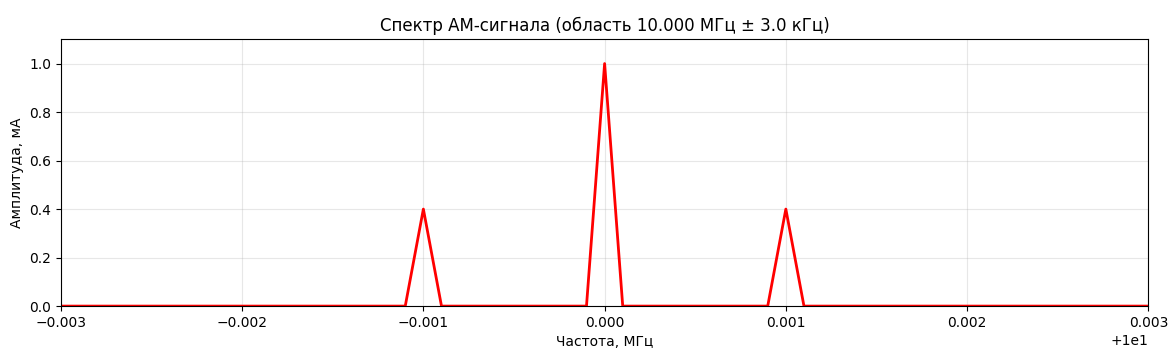
\includegraphics[width=0.8\textwidth]{pick7.png}
    \caption{Спектр Амплитудно-модулированного сигнала область 10 МГц $\pm$ 3 КГц}
    \label{fig:example}
\end{figure}



\end{document}